% ================================================================
% The Retrieve and Connect version of latex/starters/retrieval/KS3/solvingEquationsStarters_workedSolutions.tex
%
% This is the same deck as the one above, made by renaming the titles in it.
% Every slide that was a numbered starter is now titled
% "Retrieve and Connect", and the word is renamed wherever else a title
% used it. Nothing outside a title has been changed.
%
%   made from           latex/starters/retrieval/KS3/solvingEquationsStarters_workedSolutions.tex
%   retitling rules     version 1
%
% Please don't edit this file. It is written again from the one it was
% made from whenever that changes, so an edit here would be lost - edit
% that file instead and this one follows.
% ================================================================
% Root file used ashow macros
\documentclass{beamer}
\usepackage{tikz}
\usetikzlibrary{calc, arrows.meta, decorations.pathreplacing}
\usepackage{pgfplots}
\pgfplotsset{compat=1.18}
\usepackage{xcolor}
\usepackage{multicol}
\usepackage{amsmath}
\usepackage{amssymb}
\usepackage{textcomp} % for \texteuro

% ================================================================
% Retrieval starters for a Year 8 top set, used across the solving
% equations unit.
%
% Every starter draws on each of the four earlier topics: fractions,
% decimals and percentages; percentages with multipliers, including
% simple and compound interest; money problems, best buys and currency
% conversion, including conversion graphs; and the laws of indices,
% including fractions and decimals as the base with negative integer
% indices. Each starter uses more of the equations unit than the one
% before, in the order it is taught:
%
%   1  missing-number problems in words, such as "what number multiplied
%      by 7 makes 21?", answered by reasoning, with one written as an
%      equation; and, separately, the algebraic manipulation the unit
%      needs: collecting like terms, the index laws, expanding brackets
%      and substituting. No equation is solved formally on this starter.
%   2  one- and two-step equations, solved by doing the same thing to both
%      sides. A reverse percentage and a conversion graph read backwards
%      are one-step equations.
%   3  the unknown on both sides, and with brackets. A bar model that
%      takes the same amount from both sides, two simple interest
%      accounts on a graph, and a recurring decimal as an equation.
%   4  the unknown in the denominator: multiply both sides by it. The
%      price per roll in a best buy, a bill shared equally, and
%      x^-1 = 1/x.
%   5  equations with algebraic fractions. A car that loses a quarter of
%      its value each year, and a fraction-of-an-amount problem on a bar
%      model split into twelfths.
%   6  simultaneous equations. Two receipts, simple interest from a
%      table, two bureaux de change, and the index laws.
%
% Every starter has equations for pupils to form from a context. There
% are no quadratic equations.
%
% The methods follow the ones the class was taught:
%   - Equations are solved by doing the same thing to both sides, never
%     with a flow chart. The working is set out with the operation written
%     under both sides. Starter 2 gives the operations, starter 4 gives the
%     new one (multiplying both sides by the unknown), and starter 5 leaves
%     them blank.
%   - Compound interest and compound decrease are shown with flow charts.
%     Interest is never shown with a bar model.
%   - Division by a decimal is done with equivalent fractions, for
%     example 36 / 0.8 = 360 / 8 = 45.
%   - A decimal base is written as a simplified fraction before a
%     negative index is used, and a negative index turns the fraction
%     upside down.
%   - A recurring decimal is turned into a fraction by the algebraic
%     method only.
%
% The questions are worded as briefly as possible. Within each starter
% they run from retrieval of the earlier topics to the new idea, and the
% last question on each starter is a challenge.
% ================================================================

\setbeamertemplate{navigation symbols}{}
\setbeamersize{text margin left=0.4cm, text margin right=0.4cm}
\setlength{\multicolsep}{3pt}
\setlength{\columnsep}{16pt}

% ================================================================
% Answer-overlay helpers
% ================================================================
\newcommand{\ablank}[1]{%
  \alt<2>{\textcolor{red}{#1}}{\underline{\phantom{#1}}}%
}
\newcommand{\ashow}[1]{\uncover<2->{\textcolor{red}{\small #1}}}
\newcommand{\ashowq}[1]{\alt<2->{\textcolor{red}{\small #1}}{?}}

% Answers drawn straight on to a TikZ diagram, revealed on overlay 2 like \ashow.
% Space is reserved on overlay 1, so the diagram does not move between slides.
\usetikzlibrary{overlay-beamer-styles}
\tikzset{
  ans/.style     = {red, thick, visible on=<2->},
  ansfill/.style = {red!15, visible on=<2->},
  anslab/.style  = {red, font=\tiny, visible on=<2->},
}

% Used by the worked solutions rather than by this deck, so that each worked
% solution is first a question with room to write in and then the answer.
\newlength{\aworkpad}
\setlength{\aworkpad}{8mm}
\newcommand{\awork}[1]{%
  \par\vspace{\aworkpad}%
  \uncover<2->{#1}%
  \par\vspace{\aworkpad}%
}

% Every question list on these slides is tight, so that the diagram column and
% the question column both finish inside the slide.
\newcommand{\tightlist}{%
  \setlength{\itemsep}{0pt}\setlength{\parskip}{0pt}\setlength{\topsep}{0pt}%
}

% ================================================================
% The pictures these starters are built from.
% ================================================================
\tikzset{
  dhead/.style  = {font=\scriptsize\bfseries, anchor=west},
  vans/.style   = {anslab, font=\scriptsize},
  brace/.style  = {decorate, decoration={brace, amplitude=3pt}},
  mbrace/.style = {decorate, decoration={brace, mirror, amplitude=3pt}},
  bcell/.style  = {draw, fill=blue!6},
  bpart/.style  = {draw, fill=orange!12},
}

% Solving an equation by doing the same thing to both sides. The lines of the
% equation are lined up on the equals sign. Between two lines, \bsop writes the
% operation under both sides, and \bsopgap leaves it as a blank to fill in.
%   \begin{bothsides}{Working for Q4}
%     4x-7 & = & 29\\  \bsop{+7}  4x & = & \ablank{36}\\ ...
%   \end{bothsides}
\newenvironment{bothsides}[1]
  {\par{\scriptsize\bfseries #1}\par\vspace{0.1em}\footnotesize
   \hspace*{0.5cm}$\renewcommand{\arraystretch}{1.15}\begin{array}{@{}r@{\;}c@{\;}l@{}}}
  {\end{array}$\par}
\newcommand{\bsopstyle}[1]{\text{\scriptsize\color{blue!55!black}$#1$}}
\newcommand{\bsop}[1]{\bsopstyle{#1} & & \bsopstyle{#1}\\}
\newcommand{\bsopgap}[1]{\text{\scriptsize\ablank{$#1$}} & & \text{\scriptsize\ablank{$#1$}}\\}

% Flow charts, for compound interest and compound decrease only. The chain runs
% forwards along the top, with one multiplier on each arrow. \flowback draws the
% way back underneath, from right to left, with a division on each arrow. The
% arrow labels have a fixed height, so that an answer revealed on an arrow does
% not move the rest of the slide.
\tikzset{
  fbox/.style   = {draw, rounded corners=2pt, minimum width=0.9cm,
                   inner sep=1pt, font=\footnotesize, text height=2.2ex, text depth=0.9ex},
  farrow/.style = {-{Stealth[length=4pt]}, thick},
  barrow/.style = {-{Stealth[length=4pt]}, thick, gray!70!black, bend left=40},
  flab/.style   = {font=\scriptsize, inner sep=1.5pt, text height=1.6ex, text depth=0.5ex},
}
% \flowchart{name}{box 1}{op 1}{box 2}{op 2}{box 3}
\newcommand{\flowchart}[6]{%
  \node[fbox] (#1a) at (0.45,0) {#2};
  \node[fbox] (#1b) at (2.1,0)  {#4};
  \node[fbox] (#1c) at (3.75,0) {#6};
  \draw[farrow] (#1a) -- node[flab, above] {#3} (#1b);
  \draw[farrow] (#1b) -- node[flab, above] {#5} (#1c);
}
% \flowback{name}{back op 2}{back op 1}
\newcommand{\flowback}[3]{%
  \draw[barrow] (#1c.south) to node[flab, below] {#2} (#1b.south);
  \draw[barrow] (#1b.south) to node[flab, below] {#3} (#1a.south);
}

% Graphs: a light grid, small tick labels, and the axis labels pulled in
% close so that the graph fits the diagram column.
\pgfplotsset{
  startergraph/.style = {
    scale only axis, width=3.2cm,
    grid=both, grid style={black!12}, axis lines=left,
    tick label style={font=\tiny}, label style={font=\scriptsize},
    xlabel style={yshift=4pt}, ylabel style={yshift=-6pt},
  },
}

% A receipt from a café, drawn with a torn bottom edge.
% \receipt{x}{first line}{second line}{total}, with its top-left corner at (x,0)
\newcommand{\receipt}[4]{%
  \draw[fill=yellow!4, draw=black!60]
    (#1,0) -- ({#1+1.95},0) -- ({#1+1.95},-1.3)
    \foreach \i in {1,...,6} { -- ({#1+1.95-0.325*\i+0.1625},-1.38) -- ({#1+1.95-0.325*\i},-1.3) }
    -- cycle;
  \node[anchor=west] at ({#1+0.1},-0.25) {#2};
  \node[anchor=west] at ({#1+0.1},-0.58) {#3};
  \draw[black!50, dashed] ({#1+0.1},-0.8) -- ({#1+1.85},-0.8);
  \node[anchor=west, font=\scriptsize\bfseries] at ({#1+0.1},-1.05) {Total};
  \node[anchor=east] at ({#1+1.85},-1.05) {#4};
}

\title{Solving Equations: Retrieve and Connects}
\author{}
\date{}

\begin{document}

\frame{\titlepage}

\begin{frame}{Contents}
\small
\begin{columns}[T]
\begin{column}{0.5\textwidth}
\textbf{Questions and short answers}
\begin{itemize}
\item \hyperlink{q-st1}{\beamergotobutton{Retrieve and Connect 1}}
\item \hyperlink{q-st2}{\beamergotobutton{Retrieve and Connect 2}}
\item \hyperlink{q-st3}{\beamergotobutton{Retrieve and Connect 3}}
\item \hyperlink{q-st4}{\beamergotobutton{Retrieve and Connect 4}}
\item \hyperlink{q-st5}{\beamergotobutton{Retrieve and Connect 5}}
\item \hyperlink{q-st6}{\beamergotobutton{Retrieve and Connect 6}}
\end{itemize}
\end{column}
\begin{column}{0.5\textwidth}
\textbf{Worked solutions}
\begin{itemize}
\item \hyperlink{work-st1}{\beamergotobutton{Retrieve and Connect 1}}
\item \hyperlink{work-st2}{\beamergotobutton{Retrieve and Connect 2}}
\item \hyperlink{work-st3}{\beamergotobutton{Retrieve and Connect 3}}
\item \hyperlink{work-st4}{\beamergotobutton{Retrieve and Connect 4}}
\item \hyperlink{work-st5}{\beamergotobutton{Retrieve and Connect 5}}
\item \hyperlink{work-st6}{\beamergotobutton{Retrieve and Connect 6}}
\end{itemize}
\end{column}
\end{columns}
\end{frame}

%------------------------------------------------------------------
% STARTER 1
%------------------------------------------------------------------
\begin{frame}[t]{Retrieve and Connect: Missing Numbers \& Expressions}
\hypertarget{q-st1}{}
\begin{columns}[T,onlytextwidth]

\column{0.36\textwidth}
\vspace{-0.4em}
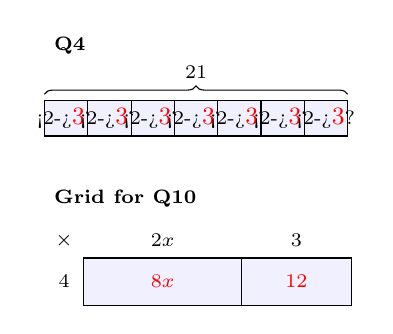
\begin{tikzpicture}[every node/.style={font=\scriptsize}]

% ---- Bar model for Q4: 21 split into 7 equal parts. One part is 0.55 cm. ----
\node[dhead] at (0,1.15) {Q4};
\begin{scope}[x=0.55cm]
% --- Q4 answer: each of the 7 parts is 3 ---
\foreach \i in {0,...,6} {
  \draw[bcell] (\i,0) rectangle ({\i+1},0.45);
  \node at ({\i+0.5},0.225) {\ashowq{3}};}
\draw[brace] (0,0.53) -- (7,0.53) node[midway, above=2pt] {$21$};
\end{scope}

% ---- Grid for expanding 4(2x + 3) in Q10 ----
\begin{scope}[yshift=-1.55cm]
\node[dhead] at (0,0.75) {Grid for Q10};
\node at (0.25,0.22) {$\times$};
\node at (1.5,0.22)  {$2x$};
\node at (3.2,0.22)  {$3$};
\node at (0.25,-0.3) {$4$};
\draw[bcell] (0.5,-0.6) rectangle (2.5,0);
\draw[bcell] (2.5,-0.6) rectangle (3.9,0);
% --- Q10 answer: the two parts of the expansion ---
\node[vans] at (1.5,-0.3) {$8x$};
\node[vans] at (3.2,-0.3) {$12$};
\end{scope}

\end{tikzpicture}

\column{0.64\textwidth}
\vspace{-1.5em}
\footnotesize
\begin{enumerate}\tightlist
{\setlength{\columnsep}{12pt}%
\begin{multicols}{3}
  \item $\tfrac25=$ \ablank{$40\%$}
  \columnbreak
  \item $3^{-2}$ \ashow{$=\tfrac19$}
  \columnbreak
  \item $0.2^{-1}$ \ashow{$=\left(\tfrac15\right)^{-1}=5$}
\end{multicols}}
  \item What number multiplied by $7$ makes $21$?
        \ashow{$3$}
  \item What number plus $8$ makes $3$?
        \ashow{$-5$}
  \item What number multiplied by $1.2$ makes $60$?
        \ashow{$\tfrac{60}{1.2}=\tfrac{600}{12}=50$}
  \item How many \pounds1.50 tickets can \pounds12 buy?
        \ashow{$\tfrac{12}{1.5}=\tfrac{120}{15}=8$}
  \item[] \vspace{2pt}Simplify the expressions below:
\begin{multicols}{2}
  \item $3a+5b-a+2b$ \ashow{$2a+7b$}
  \columnbreak
  \item $2a\times3a^4$ \ashow{$6a^5$}
\end{multicols}
  \item Expand $4(2x+3)$ using the grid.
        \ashow{$8x+12$}
  \item Expand and simplify $3(x+2)-2(x-1)$.
        \ashow{$3x+6-2x+2=x+8$}
  \item Find $5-3x$ when $x=-2$.
        \ashow{$5-3\times(-2)=11$}
  \item (Challenge) Think of a number, double it and add $6$. Halve the result, then
        subtract the number you started with. Show with algebra that you always get $3$.
        \ashow{$\tfrac{2x+6}{2}-x=x+3-x=3$}
\end{enumerate}
\end{columns}
\end{frame}

% Worked solutions for Starter 1
\begin{frame}[t]{Worked Solution: Retrieve and Connect 1, Question 1}
\hypertarget{work-st1}{}
\textbf{Question:} $\frac25 = ?$ as a percentage.
\awork{Solution: 
\[
\frac25 = \frac{2\times20}{5\times20} = \frac{40}{100} = 40\%.
\]
Multiply numerator and denominator by 20 to make the denominator 100.
}
\end{frame}

\begin{frame}[t]{Worked Solution: Retrieve and Connect 1, Question 2}
\textbf{Question:} $3^{-2} = ?$
\awork{Solution: 
\[
3^{-2} = \frac{1}{3^2} = \frac{1}{9}.
\]
A negative index means take the reciprocal.
}
\end{frame}

\begin{frame}[t]{Worked Solution: Retrieve and Connect 1, Question 3}
\textbf{Question:} $0.2^{-1} = ?$
\awork{Solution: 
\[
0.2 = \frac{2}{10} = \frac15, \quad \text{so} \quad 0.2^{-1} = \left(\frac15\right)^{-1} = 5.
\]
Write the decimal as a fraction, then flip it.
}
\end{frame}

\begin{frame}[t]{Worked Solution: Retrieve and Connect 1, Question 4}
\textbf{Question:} What number multiplied by $7$ makes $21$?
\awork{Solution: Let the number be $x$. Then
\[
7x = 21.
\]
Divide both sides by $7$:
\[
x = \frac{21}{7} = 3.
\]
So the number is $3$.
}
\end{frame}

\begin{frame}[t]{Worked Solution: Retrieve and Connect 1, Question 5}
\textbf{Question:} What number plus $8$ makes $3$?
\awork{Solution: Let the number be $x$. Then
\[
x + 8 = 3.
\]
Subtract $8$ from both sides:
\[
x = 3 - 8 = -5.
\]
So the number is $-5$.
}
\end{frame}

\begin{frame}[t]{Worked Solution: Retrieve and Connect 1, Question 6}
\textbf{Question:} What number multiplied by $1.2$ makes $60$?
\awork{Solution: Let the number be $x$. Then
\[
1.2x = 60.
\]
Divide both sides by $1.2$:
\[
x = \frac{60}{1.2} = \frac{600}{12} = 50.
\]
So the number is $50$.
}
\end{frame}

\begin{frame}[t]{Worked Solution: Retrieve and Connect 1, Question 7}
\textbf{Question:} How many \pounds1.50 tickets can \pounds12 buy?
\awork{Solution: Let $n$ be the number of tickets. Then
\[
1.5n = 12.
\]
Divide both sides by $1.5$:
\[
n = \frac{12}{1.5} = \frac{120}{15} = 8.
\]
So $8$ tickets can be bought.
}
\end{frame}

\begin{frame}[t]{Worked Solution: Retrieve and Connect 1, Question 8}
\textbf{Question:} Simplify $3a+5b-a+2b$.
\awork{Solution: Collect like terms:
\[
3a - a = 2a, \qquad 5b + 2b = 7b.
\]
So the simplified expression is
\[
2a + 7b.
\]
}
\end{frame}

\begin{frame}[t]{Worked Solution: Retrieve and Connect 1, Question 9}
\textbf{Question:} Simplify $2a\times3a^4$.
\awork{Solution: Multiply the coefficients and the powers of $a$:
\[
2a \times 3a^4 = (2\times3) \times (a^1 \times a^4) = 6a^{1+4} = 6a^5.
\]
}
\end{frame}

\begin{frame}[t]{Worked Solution: Retrieve and Connect 1, Question 10}
\textbf{Question:} Expand $4(2x+3)$ using the grid.
\awork{Solution: Using the grid:
\[
4 \times 2x = 8x, \qquad 4 \times 3 = 12.
\]
So
\[
4(2x+3) = 8x + 12.
\]
}
\end{frame}

\begin{frame}[t]{Worked Solution: Retrieve and Connect 1, Question 11}
\textbf{Question:} Expand and simplify $3(x+2)-2(x-1)$.
\awork{Solution: Expand each bracket:
\[
3(x+2) = 3x + 6, \qquad -2(x-1) = -2x + 2.
\]
Add the results:
\[
3x + 6 - 2x + 2 = x + 8.
\]
}
\end{frame}

\begin{frame}[t]{Worked Solution: Retrieve and Connect 1, Question 12}
\textbf{Question:} Find $5-3x$ when $x=-2$.
\awork{Solution: Substitute $x=-2$:
\[
5 - 3(-2) = 5 + 6 = 11.
\]
}
\end{frame}

\begin{frame}[t]{Worked Solution: Retrieve and Connect 1, Question 13}
\textbf{Question:} (Challenge) Think of a number, double it and add $6$. Halve the result, then subtract the number you started with. Show with algebra that you always get $3$.
\awork{Solution: Let the starting number be $x$.
\[
\text{Double it: } 2x, \qquad \text{add }6: 2x+6.
\]
Halve the result:
\[
\frac{2x+6}{2} = x+3.
\]
Subtract the original number:
\[
(x+3) - x = 3.
\]
So the final result is always $3$.
}
\end{frame}

%------------------------------------------------------------------
% STARTER 2
%------------------------------------------------------------------
\begin{frame}[t]{Retrieve and Connect: One- \& Two-Step Equations}
\hypertarget{q-st2}{}
\begin{columns}[T,onlytextwidth]

\column{0.36\textwidth}
\vspace{-0.4em}
% --- Q4 answer: the right-hand side of each line ---
\begin{bothsides}{Working for Q4}
  4x-7 & = & 29\\
  \bsop{+7}
  4x   & = & \ablank{36}\\
  \bsop{\div4}
  x    & = & \ablank{9}
\end{bothsides}

\vspace{0.3em}
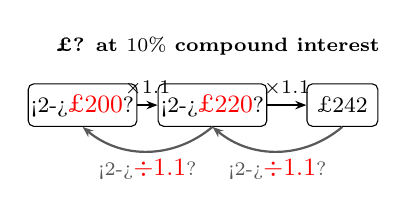
\begin{tikzpicture}[every node/.style={font=\scriptsize}]
% ---- Compound interest at 10% a year, for 2 years ----
\node[dhead] at (0,0.75) {\pounds? at $10\%$ compound interest};
% --- Q8 answer: 242 / 1.1 = 220, and 220 / 1.1 = 200 ---
\flowchart{b}{\ashowq{\pounds200}}{$\times1.1$}{\ashowq{\pounds220}}{$\times1.1$}{\pounds242}
\flowback{b}{\ashowq{$\div1.1$}}{\ashowq{$\div1.1$}}
\end{tikzpicture}

\vspace{0.1em}
{\scriptsize\bfseries Conversion graph}\par
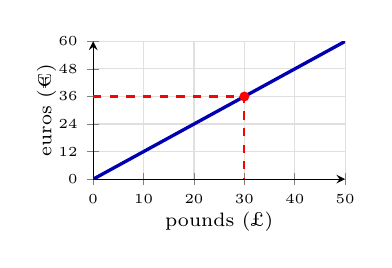
\begin{tikzpicture}
\begin{axis}[startergraph, height=1.75cm,
  xmin=0, xmax=50, ymin=0, ymax=60,
  xtick={0,10,...,50}, ytick={0,12,...,60},
  xlabel={pounds (\pounds)}, ylabel={euros (\texteuro)},
]
  \addplot[blue!70!black, very thick, domain=0:50] {1.2*x};
  % --- Q9 answer: across from 36 euros to the line, and down to 30 pounds ---
  \draw[ans, dashed] (axis cs:0,36) -- (axis cs:30,36) -- (axis cs:30,0);
  \fill[ans] (axis cs:30,36) circle (1.8pt);
\end{axis}
\end{tikzpicture}

\column{0.64\textwidth}
\vspace{-1.5em}
\footnotesize
\begin{enumerate}\tightlist
{\setlength{\columnsep}{12pt}%
\begin{multicols}{3}
  \item $\tfrac38=$ \ablank{$37.5$}$\%$
  \columnbreak
  \item $2^{-3}$ \ashow{$=\tfrac18$}
  \columnbreak
  \item $0.5^{-2}$ \ashow{$=\left(\tfrac12\right)^{-2}=2^2=4$}
\end{multicols}}
  \item I think of a number $x$, multiply it by $4$ and subtract $7$ to get $29$. Write an
        equation, then complete the working on the left.
        \ashow{$4x-7=29$}
  \item[] Solve each equation.
\begin{multicols}{2}
  \item $3x+5=26$\\ \ashow{$3x=21$, \; $x=7$}
  \columnbreak
  \item $7-2x=15$\\ \ashow{$-2x=8$, \; $x=-4$}
\end{multicols}
  \item Complete the sentence: a reduction by $20\%$ leaves $80\%$ of the original amount. To find the amount after the reduction we multiply the original by \ablank{$0.8$}.
  \item A price falls by $20\%$ to \pounds36. Solve an equation to find the original
        price, \pounds$p$.
        \ashow{$0.8p=36$, \; $p=\tfrac{36}{0.8}=\tfrac{360}{8}=45$}
  \vspace{2pt}\item Complete the flow chart. How much was invested?
        \ashow{$\tfrac{242}{1.1}=\tfrac{2420}{11}=220$, \; $\tfrac{2200}{11}=200$}
  \vspace{2pt}\item Use the graph to change \texteuro36 into pounds. Check by solving $1.2x=36$.
        \ashow{\pounds30; \; $x=\tfrac{360}{12}=30$}
  \item (Challenge) Solve $2^{x+4}=\tfrac18$.
        \ashow{$2^{x+4}=2^{-3}$, \; $x+4=-3$, \; $x=-7$}
\end{enumerate}
\end{columns}
\end{frame}

% Worked solutions for Starter 2
\begin{frame}[t]{Worked Solution: Retrieve and Connect 2, Question 1}
\hypertarget{work-st2}{}
\textbf{Question:} $\frac38 = ?\%$
\awork{Solution: 
\[
\frac38 = 0.375 = 37.5\%.
\]
Or multiply by $100$:
\[
\frac38 \times 100 = \frac{300}{8} = 37.5.
\]
So $\frac38 = 37.5\%$.
}
\end{frame}

\begin{frame}[t]{Worked Solution: Retrieve and Connect 2, Question 2}
\textbf{Question:} $2^{-3} = ?$
\awork{Solution: 
\[
2^{-3} = \frac{1}{2^3} = \frac{1}{8}.
\]
}
\end{frame}

\begin{frame}[t]{Worked Solution: Retrieve and Connect 2, Question 3}
\textbf{Question:} $0.5^{-2} = ?$
\awork{Solution: 
\[
0.5 = \frac12, \quad \text{so} \quad 0.5^{-2} = \left(\frac12\right)^{-2} = 2^2 = 4.
\]
}
\end{frame}

\begin{frame}[t]{Worked Solution: Retrieve and Connect 2, Question 4}
\textbf{Question:} I think of a number $x$, multiply it by $4$ and subtract $7$ to get $29$. Write an equation, then complete the working on the left.
\awork{Solution: The equation is
\[
4x - 7 = 29.
\]
Add $7$ to both sides:
\[
4x = 36.
\]
Divide both sides by $4$:
\[
x = 9.
\]
}
\end{frame}

\begin{frame}[t]{Worked Solution: Retrieve and Connect 2, Question 5}
\textbf{Question:} Solve $3x+5=26$.
\awork{Solution: 
\[
3x + 5 = 26.
\]
Subtract $5$:
\[
3x = 21.
\]
Divide by $3$:
\[
x = 7.
\]
}
\end{frame}

\begin{frame}[t]{Worked Solution: Retrieve and Connect 2, Question 6}
\textbf{Question:} Solve $7-2x=15$.
\awork{Solution: 
\[
7 - 2x = 15.
\]
Subtract $7$:
\[
-2x = 8.
\]
Divide by $-2$:
\[
x = -4.
\]
}
\end{frame}

\begin{frame}[t]{Worked Solution: Retrieve and Connect 2, Question 7}
\textbf{Question:} Complete the sentence: a reduction by $20\%$ leaves $80\%$ of the original amount. To find the amount after the reduction we multiply the original by \ablank{$0.8$}.
\awork{Solution: The multiplier is
\[
1 - 0.20 = 0.80 = 0.8.
\]
So we multiply the original by $0.8$.
}
\end{frame}

\begin{frame}[t]{Worked Solution: Retrieve and Connect 2, Question 8}
\textbf{Question:} A price falls by $20\%$ to \pounds36. Solve an equation to find the original price, \pounds$p$.
\awork{Solution: After a $20\%$ reduction, the price is $80\%$ of the original. So
\[
0.8p = 36.
\]
Divide both sides by $0.8$:
\[
p = \frac{36}{0.8} = \frac{360}{8} = 45.
\]
So the original price was \pounds45.
}
\end{frame}

\begin{frame}[t]{Worked Solution: Retrieve and Connect 2, Question 9}
\textbf{Question:} Complete the flow chart. How much was invested?
\awork{Solution: The flow chart shows an amount multiplied by $1.1$ twice to get \pounds242. Work backwards:
\[
242 \div 1.1 = \frac{242}{1.1} = \frac{2420}{11} = 220,
\]
\[
220 \div 1.1 = \frac{220}{1.1} = \frac{2200}{11} = 200.
\]
So \pounds200 was invested.
}
\end{frame}

\begin{frame}[t]{Worked Solution: Retrieve and Connect 2, Question 10}
\textbf{Question:} Use the graph to change \texteuro36 into pounds. Check by solving $1.2x=36$.
\awork{Solution: From the graph, \texteuro36 corresponds to \pounds30. Check:
\[
1.2x = 36 \Rightarrow x = \frac{36}{1.2} = \frac{360}{12} = 30.
\]
So \texteuro36 is \pounds30.
}
\end{frame}

\begin{frame}[t]{Worked Solution: Retrieve and Connect 2, Question 11}
\textbf{Question:} (Challenge) Solve $2^{x+4}=\frac18$.
\awork{Solution: Write $\frac18 = 2^{-3}$. Then
\[
2^{x+4} = 2^{-3}.
\]
Since the bases are the same, equate the exponents:
\[
x + 4 = -3.
\]
Subtract $4$:
\[
x = -7.
\]
}
\end{frame}

%------------------------------------------------------------------
% STARTER 3
%------------------------------------------------------------------
\begin{frame}[t]{Retrieve and Connect: Unknowns on Both Sides}
\hypertarget{q-st3}{}
\begin{columns}[T,onlytextwidth]

\column{0.36\textwidth}
\vspace{-0.4em}
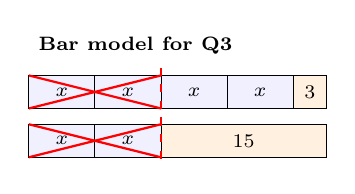
\begin{tikzpicture}[every node/.style={font=\scriptsize}]

% ---- Bar model for 4x + 3 = 2x + 15, drawn to scale. One unit is 0.14 cm, so
% x = 6 is 0.84 cm and both bars are 27 units long. ----
\node[dhead] at (0,0.8) {Bar model for Q3};
\begin{scope}[x=0.14cm]
\foreach \i in {0,...,3} {
  \draw[bcell] ({6*\i},0) rectangle ({6*\i+6},0.42);
  \node at ({6*\i+3},0.21) {$x$};}
\draw[bpart] (24,0) rectangle (27,0.42);
\node at (25.5,0.21) {$3$};
\foreach \i in {0,1} {
  \draw[bcell] ({6*\i},-0.62) rectangle ({6*\i+6},-0.2);
  \node at ({6*\i+3},-0.41) {$x$};}
\draw[bpart] (12,-0.62) rectangle (27,-0.2);
\node at (19.5,-0.41) {$15$};
% --- Q3 answer: 2x is taken from both bars, which leaves 2x + 3 = 15 ---
\foreach \y in {0,-0.62} {
  \draw[ans] (0,\y) -- (12,{\y+0.42});
  \draw[ans] (0,{\y+0.42}) -- (12,\y);}
\draw[ans, dashed] (12,0.52) -- (12,-0.72);
\end{scope}

\end{tikzpicture}

\vspace{0.5em}
{\scriptsize\bfseries Graph for Q6 and Q7}\par
\vspace{-0.1em}
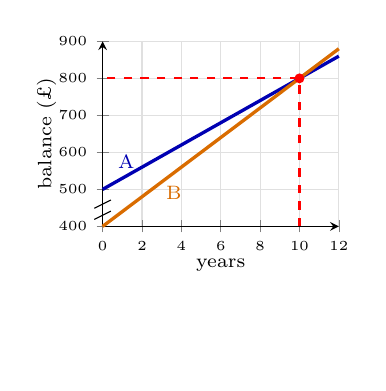
\begin{tikzpicture}
\begin{axis}[startergraph, width=3.0cm, height=2.35cm,
  xmin=0, xmax=12, ymin=400, ymax=900,
  xtick={0,2,...,12}, ytick={400,500,...,900},
  xlabel={years}, ylabel={balance (\pounds)}, clip=false,
]
  % The y-axis starts at 400 pounds, so it is drawn with a break near the bottom.
  \fill[white] ($(rel axis cs:0,0.06)+(-3pt,0)$) rectangle ($(rel axis cs:0,0.12)+(3pt,0)$);
  \draw ($(rel axis cs:0,0.06)+(-3pt,-1.5pt)$) -- ++(6pt,3pt);
  \draw ($(rel axis cs:0,0.12)+(-3pt,-1.5pt)$) -- ++(6pt,3pt);
  \addplot[blue!70!black, very thick, domain=0:12] {500+30*x}
    node[pos=0.1, above, font=\scriptsize, inner sep=2pt] {A};
  \addplot[orange!85!black, very thick, domain=0:12] {400+40*x}
    node[pos=0.25, below right, font=\scriptsize, inner sep=1pt] {B};
  % --- Q7 answer: the lines cross after 10 years, at 800 pounds ---
  \draw[ans, dashed] (axis cs:10,400) -- (axis cs:10,800) -- (axis cs:0,800);
  \fill[ans] (axis cs:10,800) circle (1.8pt);
\end{axis}
\end{tikzpicture}

\column{0.64\textwidth}
\vspace{-1.5em}
\footnotesize
\begin{enumerate}\tightlist
\begin{multicols}{2}
  \item What is $0.45$ as a fraction?
        \ashow{$\tfrac{45}{100}=\tfrac{9}{20}$}
  \columnbreak
  \item Simplify $3x^{-2}\times4x^5$
        \ashow{$12x^3$}
\end{multicols}
  \item Use the bar model to solve $4x+3=2x+15$.
        \ashow{Take $2x$ from both sides: \; $2x+3=15$, \; $x=6$}
  \item[] Solve each equation below:
\begin{multicols}{2}
  \item $7x-4=3x+24$ \ashow{$4x-4=24$, \; $x=7$}
  \columnbreak
  \item $6(x-2)=2x+8$ \ashow{$6x-12=2x+8$, \; $x=5$}
\end{multicols}
  \item A has \pounds500 at $6\%$ and B has \pounds400 at $10\%$ simple interest a year.
        Write each balance after $n$ years.
        \ashow{A: $500+30n$, \; B: $400+40n$}
  \item When are the balances equal? Solve an equation, then check on the graph.
        \ashow{$500+30n=400+40n$, \; $100=10n$, \; $n=10$}
\begin{multicols}{2}
  \item Solve $7^{3x}=7^{x+8}$
        \ashow{$3x=x+8$, \; $x=4$}
  \columnbreak
  \item What is \pounds250 in euros, at \texteuro1.16 per \pounds1
        \ashow{\texteuro290}
\end{multicols}
  \item (Challenge) $x=0.\dot7$. Use $10x-x$ to write $x$ as a fraction.
        \ashow{$10x=7.\dot7$, \; $9x=7$, \; $x=\tfrac79$}
\end{enumerate}
\end{columns}
\end{frame}

% Worked solutions for Starter 3
\begin{frame}[t]{Worked Solution: Retrieve and Connect 3, Question 1}
\hypertarget{work-st3}{}
\textbf{Question:} What is $0.45$ as a fraction?
\awork{Solution: 
\[
0.45 = \frac{45}{100} = \frac{9}{20}.
\]
}
\end{frame}

\begin{frame}[t]{Worked Solution: Retrieve and Connect 3, Question 2}
\textbf{Question:} Simplify $3x^{-2}\times4x^5$.
\awork{Solution: Multiply coefficients and add indices:
\[
3 \times 4 = 12, \qquad x^{-2} \times x^5 = x^{-2+5} = x^3.
\]
So
\[
3x^{-2} \times 4x^5 = 12x^3.
\]
}
\end{frame}

\begin{frame}[t]{Worked Solution: Retrieve and Connect 3, Question 3}
\textbf{Question:} Use the bar model to solve $4x+3=2x+15$.
\awork{Solution: From the bar model, take $2x$ from both sides:
\[
4x+3 - 2x = 2x+15 - 2x \Rightarrow 2x+3 = 15.
\]
Subtract $3$:
\[
2x = 12.
\]
Divide by $2$:
\[
x = 6.
\]
}
\end{frame}

\begin{frame}[t]{Worked Solution: Retrieve and Connect 3, Question 4}
\textbf{Question:} Solve $7x-4=3x+24$.
\awork{Solution: 
\[
7x - 4 = 3x + 24.
\]
Subtract $3x$ from both sides:
\[
4x - 4 = 24.
\]
Add $4$:
\[
4x = 28.
\]
Divide by $4$:
\[
x = 7.
\]
}
\end{frame}

\begin{frame}[t]{Worked Solution: Retrieve and Connect 3, Question 5}
\textbf{Question:} Solve $6(x-2)=2x+8$.
\awork{Solution: Expand the bracket:
\[
6x - 12 = 2x + 8.
\]
Subtract $2x$:
\[
4x - 12 = 8.
\]
Add $12$:
\[
4x = 20.
\]
Divide by $4$:
\[
x = 5.
\]
}
\end{frame}

\begin{frame}[t]{Worked Solution: Retrieve and Connect 3, Question 6}
\textbf{Question:} A has \pounds500 at $6\%$ and B has \pounds400 at $10\%$ simple interest a year. Write each balance after $n$ years.
\awork{Solution: A earns $500 \times 0.06 = 30$ per year. So balance A is
\[
500 + 30n.
\]
B earns $400 \times 0.10 = 40$ per year. So balance B is
\[
400 + 40n.
\]
}
\end{frame}

\begin{frame}[t]{Worked Solution: Retrieve and Connect 3, Question 7}
\textbf{Question:} When are the balances equal? Solve an equation, then check on the graph.
\awork{Solution: Set the balances equal:
\[
500 + 30n = 400 + 40n.
\]
Subtract $400$:
\[
100 + 30n = 40n.
\]
Subtract $30n$:
\[
100 = 10n.
\]
Divide by $10$:
\[
n = 10.
\]
At $10$ years, both balances are \pounds800, which matches the graph.
}
\end{frame}

\begin{frame}[t]{Worked Solution: Retrieve and Connect 3, Question 8}
\textbf{Question:} Solve $7^{3x}=7^{x+8}$.
\awork{Solution: Bases are the same, so equate exponents:
\[
3x = x + 8.
\]
Subtract $x$:
\[
2x = 8.
\]
Divide by $2$:
\[
x = 4.
\]
}
\end{frame}

\begin{frame}[t]{Worked Solution: Retrieve and Connect 3, Question 9}
\textbf{Question:} What is \pounds250 in euros, at \texteuro1.16 per \pounds1?
\awork{Solution: Multiply:
\[
250 \times 1.16 = 250 \times (1 + 0.16) = 250 + 40 = 290.
\]
So \pounds250 is \texteuro290.
}
\end{frame}

\begin{frame}[t]{Worked Solution: Retrieve and Connect 3, Question 10}
\textbf{Question:} (Challenge) $x=0.\dot7$. Use $10x-x$ to write $x$ as a fraction.
\awork{Solution: Let $x = 0.777\ldots$. Then
\[
10x = 7.777\ldots
\]
Subtract $x$:
\[
10x - x = 7.777\ldots - 0.777\ldots = 7.
\]
So
\[
9x = 7 \Rightarrow x = \frac{7}{9}.
\]
}
\end{frame}

%------------------------------------------------------------------
% STARTER 4
%------------------------------------------------------------------
\begin{frame}[t]{Retrieve and Connect: Unknown in the Denominator}
\hypertarget{q-st4}{}
\begin{columns}[T,onlytextwidth]

\column{0.36\textwidth}
\vspace{-0.4em}
{\scriptsize\bfseries Bread rolls}\par
\vspace{0.2em}
{\scriptsize
\renewcommand{\arraystretch}{1.4}\setlength{\tabcolsep}{3.5pt}
\begin{tabular}{c|c|c|c}
  Pack & Rolls & Price & Per roll\\ \hline
  A & $4$ & \pounds1.60 & \ablank{$40$p}\\
  B & $6$ & \pounds2.10 & \ablank{$35$p}\\
  C & $n$ & \pounds3.60 & $30$p
\end{tabular}}

% --- Q5 answer: the right-hand side of the second line, and x ---
\vspace{0.4em}
\begin{bothsides}{Working for Q5}
  \dfrac{12}{x} & = & 3\\
  \bsop{\times x}
  12 & = & \ablank{3x}\\
  \bsop{\div3}
  \ablank{4} & = & x
\end{bothsides}

\vspace{0.9em}
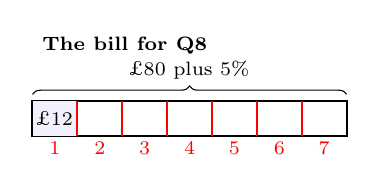
\begin{tikzpicture}[every node/.style={font=\scriptsize}]

% ---- The bill for Q8, drawn to scale: one share of 12 pounds is 0.57 cm ----
\node[dhead] at (0,1.15) {The bill for Q8};
\begin{scope}[x=0.57cm]
\draw[thick] (0,0) rectangle (7,0.45);
\draw[bcell] (0,0) rectangle (1,0.45);
\node at (0.5,0.225) {\pounds12};
\draw[brace] (0,0.53) -- (7,0.53) node[midway, above=2pt] {\pounds80 plus $5\%$};
% --- Q8 answer: the bill cut into shares of 12 pounds, one for each person ---
\foreach \i in {1,...,6} \draw[ans] (\i,0) -- (\i,0.45);
\foreach \i in {1,...,7} \node[vans, below, inner sep=2pt] at ({\i-0.5},0) {\i};
\end{scope}

\end{tikzpicture}

\column{0.64\textwidth}
\vspace{-1.5em}
\footnotesize
\begin{enumerate}\tightlist
\begin{multicols}{2}
  \item $\tfrac{7}{20}=$ \ablank{$35$}$\%$
  \columnbreak
  \item $0.4^{-2}$
        \ashow{$=\left(\tfrac25\right)^{-2}=\left(\tfrac52\right)^2=\tfrac{25}{4}$}
\end{multicols}
  \item Complete the table. Which is the better buy, A or B?
        \ashow{B}
  \item Solve an equation to find $n$ for pack C.
        \ashow{$\tfrac{360}{n}=30$, \; $360=30n$, \; $n=12$}
  \item[] \vspace{2pt}Solve each equation.
{\setlength{\columnsep}{12pt}%
\begin{multicols}{3}
  \item $\dfrac{12}{x}=3$\\[2pt] \ashow{$x=4$}
  \columnbreak
  \item $\dfrac{35}{x-2}=5$\\[2pt] \ashow{$35=5(x-2)$, \; $x=9$}
  \columnbreak
  \item $3+\dfrac{18}{x}=9$\\[2pt] \ashow{$\tfrac{18}{x}=6$, \; $x=3$}
\end{multicols}}
  \item A \pounds80 bill has $5\%$ service added, and is split equally at \pounds12 each.
        Solve an equation to find the number of people, $p$.
        \ashow{$\tfrac{84}{p}=12$, \; $84=12p$, \; $p=7$}
  \item Solve $5x^{-1}=20$.
        \ashow{$\tfrac5x=20$, \; $5=20x$, \; $x=\tfrac14$}
  \item (Challenge) Solve $\dfrac{50}{x+2}=0.8^{-2}$.\\[2pt]
        \ashow{$\left(\tfrac45\right)^{-2}=\tfrac{25}{16}$, \; $800=25(x+2)$, \; $x=30$}
\end{enumerate}
\end{columns}
\end{frame}

% Worked solutions for Starter 4
\begin{frame}[t]{Worked Solution: Retrieve and Connect 4, Question 1}
\hypertarget{work-st4}{}
\textbf{Question:} $\frac{7}{20} = ?\%$
\awork{Solution: 
\[
\frac{7}{20} = \frac{7\times5}{20\times5} = \frac{35}{100} = 35\%.
\]
}
\end{frame}

\begin{frame}[t]{Worked Solution: Retrieve and Connect 4, Question 2}
\textbf{Question:} $0.4^{-2} = ?$
\awork{Solution: 
\[
0.4 = \frac{4}{10} = \frac{2}{5}, \quad \text{so} \quad 0.4^{-2} = \left(\frac{2}{5}\right)^{-2} = \left(\frac{5}{2}\right)^2 = \frac{25}{4}.
\]
}
\end{frame}

\begin{frame}[t]{Worked Solution: Retrieve and Connect 4, Question 3}
\textbf{Question:} Complete the table. Which is the better buy, A or B?
\awork{Solution: 
Pack A: \pounds1.60 for $4$ rolls, so per roll:
\[
1.60 \div 4 = 0.40 \text{ (40p)}.
\]
Pack B: \pounds2.10 for $6$ rolls, so per roll:
\[
2.10 \div 6 = 0.35 \text{ (35p)}.
\]
Pack B is cheaper per roll, so B is the better buy.
}
\end{frame}

\begin{frame}[t]{Worked Solution: Retrieve and Connect 4, Question 4}
\textbf{Question:} Solve an equation to find $n$ for pack C.
\awork{Solution: Pack C has $n$ rolls at \pounds3.60, and costs $30$p per roll, i.e. \pounds0.30. So
\[
0.30n = 3.60.
\]
Divide by $0.30$:
\[
n = \frac{3.60}{0.30} = \frac{360}{30} = 12.
\]
So $n = 12$.
}
\end{frame}

\begin{frame}[t]{Worked Solution: Retrieve and Connect 4, Question 5}
\textbf{Question:} Solve $\frac{12}{x}=3$.
\awork{Solution: Multiply both sides by $x$:
\[
12 = 3x.
\]
Divide by $3$:
\[
x = 4.
\]
}
\end{frame}

\begin{frame}[t]{Worked Solution: Retrieve and Connect 4, Question 6}
\textbf{Question:} Solve $\frac{35}{x-2}=5$.
\awork{Solution: Multiply both sides by $x-2$:
\[
35 = 5(x-2).
\]
Divide by $5$:
\[
7 = x - 2.
\]
Add $2$:
\[
x = 9.
\]
}
\end{frame}

\begin{frame}[t]{Worked Solution: Retrieve and Connect 4, Question 7}
\textbf{Question:} Solve $3+\frac{18}{x}=9$.
\awork{Solution: Subtract $3$:
\[
\frac{18}{x} = 6.
\]
Multiply by $x$:
\[
18 = 6x.
\]
Divide by $6$:
\[
x = 3.
\]
}
\end{frame}

\begin{frame}[t]{Worked Solution: Retrieve and Connect 4, Question 8}
\textbf{Question:} A \pounds80 bill has $5\%$ service added, and is split equally at \pounds12 each. Solve an equation to find the number of people, $p$.
\awork{Solution: Total bill with service:
\[
80 \times 1.05 = 84.
\]
Split equally:
\[
\frac{84}{p} = 12.
\]
Multiply by $p$:
\[
84 = 12p.
\]
Divide by $12$:
\[
p = 7.
\]
So there are $7$ people.
}
\end{frame}

\begin{frame}[t]{Worked Solution: Retrieve and Connect 4, Question 9}
\textbf{Question:} Solve $5x^{-1}=20$.
\awork{Solution: 
\[
5x^{-1} = \frac{5}{x} = 20.
\]
Multiply by $x$:
\[
5 = 20x.
\]
Divide by $20$:
\[
x = \frac{5}{20} = \frac{1}{4}.
\]
}
\end{frame}

\begin{frame}[t]{Worked Solution: Retrieve and Connect 4, Question 10}
\textbf{Question:} (Challenge) Solve $\frac{50}{x+2}=0.8^{-2}$.
\awork{Solution: First, 
\[
0.8^{-2} = \left(\frac{4}{5}\right)^{-2} = \left(\frac{5}{4}\right)^2 = \frac{25}{16}.
\]
So
\[
\frac{50}{x+2} = \frac{25}{16}.
\]
Cross-multiply:
\[
50 \times 16 = 25(x+2).
\]
\[
800 = 25(x+2).
\]
Divide by $25$:
\[
32 = x + 2.
\]
Subtract $2$:
\[
x = 30.
\]
}
\end{frame}

%------------------------------------------------------------------
% STARTER 5
%------------------------------------------------------------------
\begin{frame}[t]{Retrieve and Connect: Equations with Fractions}
\hypertarget{q-st5}{}
\begin{columns}[T,onlytextwidth]

\column{0.36\textwidth}
\vspace{-0.4em}
% --- Q3 answer: the operations, and the right-hand side of each line ---
\begin{bothsides}{Working for Q3}
  \dfrac{x+2}{3} & = & 5\\
  \bsopgap{\times3}
  x+2 & = & \ablank{15}\\
  \bsopgap{-2}
  x   & = & \ablank{13}
\end{bothsides}

\vspace{0.6em}
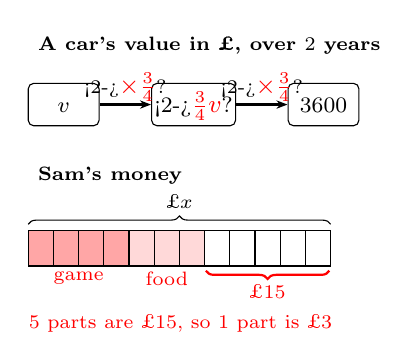
\begin{tikzpicture}[every node/.style={font=\scriptsize}]

% ---- A car that loses 25% of its value each year, for 2 years ----
\node[dhead] at (0,0.75) {A car's value in \pounds, over $2$ years};
% --- Q7 answer: the multiplier 3/4 on both arrows, and 3/4 of v after a year ---
\flowchart{c}{$v$}{\ashowq{$\times\tfrac34$}}{\ashowq{$\tfrac34v$}}%
  {\ashowq{$\times\tfrac34$}}{$3600$}

% ---- Sam's money, split into twelfths. One twelfth is 0.32 cm. ----
\begin{scope}[yshift=-2.05cm]
\node[dhead] at (0,1.15) {Sam's money};
\begin{scope}[x=0.32cm]
% --- Q8 answer: 1/3 is 4 twelfths, spent on the game, and 1/4 is 3 twelfths,
% spent on food. The 5 twelfths left are 15 pounds, so one twelfth is 3 pounds. ---
\fill[ansfill, red!35] (0,0) rectangle (4,0.45);
\fill[ansfill, red!15] (4,0) rectangle (7,0.45);
\foreach \i in {0,...,11} \draw ({\i},0) rectangle ({\i+1},0.45);
\draw[brace] (0,0.53) -- (12,0.53) node[midway, above=2pt] {\pounds$x$};
\node[vans, below, inner sep=2pt] at (2,0) {game};
\node[vans, below, inner sep=2pt] at (5.5,0) {food};
\draw[ans, mbrace] (7.05,-0.06) -- (11.95,-0.06);
\node[vans, below, inner sep=2pt] at (9.5,-0.16) {\pounds15};
\node[vans, anchor=north west, inner sep=0pt] at (0,-0.62)
  {$5$ parts are \pounds15, so $1$ part is \pounds3};
\end{scope}
\end{scope}

\end{tikzpicture}

\column{0.64\textwidth}
\vspace{-1.5em}
\footnotesize
\begin{enumerate}\tightlist
\begin{multicols}{2}
  \item $\tfrac13+\tfrac14$ \ashow{$=\tfrac{7}{12}$}
  \columnbreak
  \item $\left(\tfrac34\right)^{-2}$ \ashow{$=\left(\tfrac43\right)^2=\tfrac{16}{9}$}
\end{multicols}
  \item[] Solve each equation.
\begin{multicols}{2}
  \item $\dfrac{x+2}{3}=5$ \ashow{$x=13$}
  \columnbreak
  \item $\dfrac{2x-1}{5}=3$ \ashow{$2x-1=15$, \; $x=8$}
\end{multicols}
\vspace{3pt}
\begin{multicols}{2}
  \item $\dfrac{x}{3}+\dfrac{x}{4}=14$ \ashow{$4x+3x=168$, \; $x=24$}
  \columnbreak
  \item $\dfrac{x+3}{2}=\dfrac{x+7}{3}$ \ashow{$3(x+3)=2(x+7)$, \; $x=5$}
\end{multicols}
  \item A car loses $25\%$ of its value each year. Complete the flow chart, then solve an
        equation for $v$.
        \ashow{$\tfrac{9}{16}v=3600$, \; $9v=57\,600$, \; $v=6400$}
  \item Sam has \pounds$x$. He spends $\frac13$ on a game and $\frac14$ on food, leaving
        \pounds15. Shade the bar, then solve an equation for $x$.\\[2pt]
        \ashow{$x-\tfrac{x}{3}-\tfrac{x}{4}=15$, \; $\tfrac{5x}{12}=15$, \; $x=36$}
  \item Solve $\left(\dfrac23\right)^{x}=\dfrac94$.
        \ashow{$\left(\tfrac23\right)^{-2}=\tfrac94$, \; so $x=-2$}
  \item (Challenge) \pounds3 buys $x$ rolls and \pounds4 buys $x+4$ rolls, at the same price
        per roll. Find $x$.
        \ashow{$\tfrac{3}{x}=\tfrac{4}{x+4}$, \; $3(x+4)=4x$, \; $x=12$}
\end{enumerate}
\end{columns}
\end{frame}

% Worked solutions for Starter 5
\begin{frame}[t]{Worked Solution: Retrieve and Connect 5, Question 1}
\hypertarget{work-st5}{}
\textbf{Question:} $\frac13+\frac14$
\awork{Solution: Common denominator $12$:
\[
\frac{1}{3} + \frac{1}{4} = \frac{4}{12} + \frac{3}{12} = \frac{7}{12}.
\]
}
\end{frame}

\begin{frame}[t]{Worked Solution: Retrieve and Connect 5, Question 2}
\textbf{Question:} $\left(\frac34\right)^{-2}$
\awork{Solution: 
\[
\left(\frac{3}{4}\right)^{-2} = \left(\frac{4}{3}\right)^2 = \frac{16}{9}.
\]
}
\end{frame}

\begin{frame}[t]{Worked Solution: Retrieve and Connect 5, Question 3}
\textbf{Question:} Solve $\frac{x+2}{3}=5$.
\awork{Solution: Multiply both sides by $3$:
\[
x + 2 = 15.
\]
Subtract $2$:
\[
x = 13.
\]
}
\end{frame}

\begin{frame}[t]{Worked Solution: Retrieve and Connect 5, Question 4}
\textbf{Question:} Solve $\frac{2x-1}{5}=3$.
\awork{Solution: Multiply both sides by $5$:
\[
2x - 1 = 15.
\]
Add $1$:
\[
2x = 16.
\]
Divide by $2$:
\[
x = 8.
\]
}
\end{frame}

\begin{frame}[t]{Worked Solution: Retrieve and Connect 5, Question 5}
\textbf{Question:} Solve $\frac{x}{3}+\frac{x}{4}=14$.
\awork{Solution: Common denominator $12$:
\[
\frac{4x}{12} + \frac{3x}{12} = \frac{7x}{12} = 14.
\]
Multiply by $12$:
\[
7x = 168.
\]
Divide by $7$:
\[
x = 24.
\]
}
\end{frame}

\begin{frame}[t]{Worked Solution: Retrieve and Connect 5, Question 6}
\textbf{Question:} Solve $\frac{x+3}{2}=\frac{x+7}{3}$.
\awork{Solution: Cross-multiply:
\[
3(x+3) = 2(x+7).
\]
Expand:
\[
3x + 9 = 2x + 14.
\]
Subtract $2x$:
\[
x + 9 = 14.
\]
Subtract $9$:
\[
x = 5.
\]
}
\end{frame}

\begin{frame}[t]{Worked Solution: Retrieve and Connect 5, Question 7}
\textbf{Question:} A car loses $25\%$ of its value each year. Complete the flow chart, then solve an equation for $v$.
\awork{Solution: The multiplier for a $25\%$ loss is $1 - 0.25 = 0.75 = \frac34$. After two years:
\[
v \times \frac34 \times \frac34 = v \times \frac{9}{16} = 3600.
\]
So
\[
\frac{9}{16}v = 3600.
\]
Multiply by $16$:
\[
9v = 57600.
\]
Divide by $9$:
\[
v = 6400.
\]
So the initial value was \pounds6400.
}
\end{frame}

\begin{frame}[t]{Worked Solution: Retrieve and Connect 5, Question 8}
\textbf{Question:} Sam has \pounds$x$. He spends $\frac13$ on a game and $\frac14$ on food, leaving \pounds15. Shade the bar, then solve an equation for $x$.
\awork{Solution: Total spent:
\[
\frac{1}{3} + \frac{1}{4} = \frac{4}{12} + \frac{3}{12} = \frac{7}{12}.
\]
Remaining:
\[
1 - \frac{7}{12} = \frac{5}{12}.
\]
So
\[
\frac{5}{12}x = 15.
\]
Multiply by $12$:
\[
5x = 180.
\]
Divide by $5$:
\[
x = 36.
\]
So Sam had \pounds36.
}
\end{frame}

\begin{frame}[t]{Worked Solution: Retrieve and Connect 5, Question 9}
\textbf{Question:} Solve $\left(\frac23\right)^{x}=\frac94$.
\awork{Solution: Note that
\[
\frac{9}{4} = \left(\frac{3}{2}\right)^2 = \left(\frac{2}{3}\right)^{-2}.
\]
So
\[
\left(\frac{2}{3}\right)^x = \left(\frac{2}{3}\right)^{-2}.
\]
Equate exponents:
\[
x = -2.
\]
}
\end{frame}

\begin{frame}[t]{Worked Solution: Retrieve and Connect 5, Question 10}
\textbf{Question:} (Challenge) \pounds3 buys $x$ rolls and \pounds4 buys $x+4$ rolls, at the same price per roll. Find $x$.
\awork{Solution: Price per roll for the first purchase:
\[
\frac{3}{x}.
\]
Price per roll for the second purchase:
\[
\frac{4}{x+4}.
\]
Since the price per roll is the same:
\[
\frac{3}{x} = \frac{4}{x+4}.
\]
Cross-multiply:
\[
3(x+4) = 4x.
\]
Expand:
\[
3x + 12 = 4x.
\]
Subtract $3x$:
\[
x = 12.
\]
}
\end{frame}

%------------------------------------------------------------------
% STARTER 6
%------------------------------------------------------------------
\begin{frame}[t]{Retrieve and Connect: Simultaneous Equations}
\hypertarget{q-st6}{}
\begin{columns}[T,onlytextwidth]

\column{0.36\textwidth}
\vspace{-0.4em}
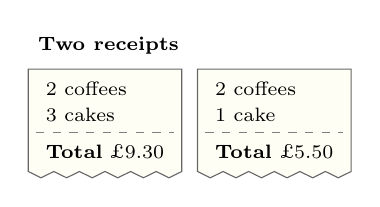
\begin{tikzpicture}[every node/.style={font=\scriptsize}]
\node[dhead] at (0,0.3) {Two receipts};
\receipt{0}{$2$ coffees}{$3$ cakes}{\pounds9.30}
\receipt{2.15}{$2$ coffees}{$1$ cake}{\pounds5.50}
\end{tikzpicture}

\vspace{0.8em}
{\scriptsize\bfseries \pounds$P$ at \pounds$I$ simple interest a year}\par
\vspace{0.2em}
{\scriptsize
\renewcommand{\arraystretch}{1.3}
\begin{tabular}{l|c|c}
  Years   & $2$        & $5$\\ \hline
  Balance & \pounds560 & \pounds650
\end{tabular}}

\vspace{0.9em}
{\scriptsize\bfseries Two bureaux de change}\par
\vspace{0.2em}
\parbox{\linewidth}{\raggedright\scriptsize
  \textbf{Airport}: no fee, and \texteuro1.10 for every \pounds1.\\[2pt]
  \textbf{High Street}: a \pounds5 fee, then \texteuro1.20 for every \pounds1 that is left.}

\column{0.64\textwidth}
\vspace{-1.5em}
\footnotesize
\begin{enumerate}\tightlist
\begin{multicols}{2}
  \item $0.125$ as a fraction
        \ashow{$\tfrac18$}
  \columnbreak
  \item $2^{-1}+2^{-2}$ as a percentage
        \ashow{$\tfrac12+\tfrac14=75\%$}
\end{multicols}
  \item Write each receipt as an equation, with $c$ for a coffee and $k$ for a cake.
        Subtract to find $k$ and $c$.
        \ashow{$2c+3k=9.30$, \; $2c+k=5.50$; \; $2k=3.80$, \; $k=1.90$, \; $c=1.80$}
  \item[] Solve each pair of equations.
\begin{multicols}{2}
  \item $\begin{aligned}[t] x+y&=10\\ x-y&=4 \end{aligned}$
        \quad\ashow{$x=7$, \; $y=3$}
  \columnbreak
  \item $\begin{aligned}[t] 2x+3y&=13\\ x+y&=5 \end{aligned}$
        \quad\ashow{$x=2$, \; $y=3$}
\end{multicols}
  \item Write two equations from the table, and solve them. Find the interest rate.
        \ashow{$P+2I=560$, \; $P+5I=650$; \; $I=30$, \; $P=500$; \; $6\%$}
  \item Write the euros, $y$, that each bureau gives for \pounds$x$. When are they equal?
        \ashow{$y=1.1x$, \; $y=1.2x-6$; \; $0.1x=6$, \; $x=\tfrac{6}{0.1}=\tfrac{60}{1}=60$}
  \item (Challenge) Solve $2^x\times2^y=64$ and $3^x\div3^y=\tfrac19$.
        \ashow{$x+y=6$, \; $x-y=-2$; \; $x=2$, \; $y=4$}
\end{enumerate}
\end{columns}
\end{frame}

% Worked solutions for Starter 6
\begin{frame}[t]{Worked Solution: Retrieve and Connect 6, Question 1}
\hypertarget{work-st6}{}
\textbf{Question:} $0.125$ as a fraction
\awork{Solution: 
\[
0.125 = \frac{125}{1000} = \frac{1}{8}.
\]
}
\end{frame}

\begin{frame}[t]{Worked Solution: Retrieve and Connect 6, Question 2}
\textbf{Question:} $2^{-1}+2^{-2}$ as a percentage
\awork{Solution: 
\[
2^{-1} = \frac{1}{2}, \qquad 2^{-2} = \frac{1}{4}.
\]
Sum:
\[
\frac{1}{2} + \frac{1}{4} = \frac{2}{4} + \frac{1}{4} = \frac{3}{4} = 75\%.
\]
}
\end{frame}

\begin{frame}[t]{Worked Solution: Retrieve and Connect 6, Question 3}
\textbf{Question:} Write each receipt as an equation, with $c$ for a coffee and $k$ for a cake. Subtract to find $k$ and $c$.
\awork{Solution: The equations are
\[
2c + 3k = 9.30 \quad (1)
\]
\[
2c + k = 5.50 \quad (2)
\]
Subtract (2) from (1):
\[
(2c+3k) - (2c+k) = 9.30 - 5.50 \Rightarrow 2k = 3.80.
\]
So
\[
k = 1.90.
\]
Substitute into (2):
\[
2c + 1.90 = 5.50 \Rightarrow 2c = 3.60 \Rightarrow c = 1.80.
\]
So a coffee is \pounds1.80 and a cake is \pounds1.90.
}
\end{frame}

\begin{frame}[t]{Worked Solution: Retrieve and Connect 6, Question 4}
\textbf{Question:} Solve $x+y=10$ and $x-y=4$.
\awork{Solution: Add the two equations:
\[
(x+y) + (x-y) = 10 + 4 \Rightarrow 2x = 14 \Rightarrow x = 7.
\]
Substitute into $x+y=10$:
\[
7 + y = 10 \Rightarrow y = 3.
\]
So $x=7$, $y=3$.
}
\end{frame}

\begin{frame}[t]{Worked Solution: Retrieve and Connect 6, Question 5}
\textbf{Question:} Solve $2x+3y=13$ and $x+y=5$.
\awork{Solution: From $x+y=5$, we have $x = 5 - y$.
Substitute into $2x+3y=13$:
\[
2(5-y) + 3y = 13.
\]
\[
10 - 2y + 3y = 13.
\]
\[
10 + y = 13 \Rightarrow y = 3.
\]
Then $x = 5 - 3 = 2$.
So $x=2$, $y=3$.
}
\end{frame}

\begin{frame}[t]{Worked Solution: Retrieve and Connect 6, Question 6}
\textbf{Question:} Write two equations from the table, and solve them. Find the interest rate.
\awork{Solution: Let $P$ be the principal and $I$ the annual interest. From the table:
\[
P + 2I = 560 \quad (1)
\]
\[
P + 5I = 650 \quad (2)
\]
Subtract (1) from (2):
\[
3I = 90 \Rightarrow I = 30.
\]
Substitute into (1):
\[
P + 60 = 560 \Rightarrow P = 500.
\]
Interest rate:
\[
\frac{I}{P} = \frac{30}{500} = 0.06 = 6\%.
\]
}
\end{frame}

\begin{frame}[t]{Worked Solution: Retrieve and Connect 6, Question 7}
\textbf{Question:} Write the euros, $y$, that each bureau gives for \pounds$x$. When are they equal?
\awork{Solution: Airport: no fee, \texteuro1.10 per \pounds1. So
\[
y = 1.1x.
\]
High Street: \pounds5 fee, then \texteuro1.20 per \pounds1 left. So
\[
y = 1.2(x - 5) = 1.2x - 6.
\]
Set equal:
\[
1.1x = 1.2x - 6.
\]
\[
6 = 0.1x.
\]
\[
x = \frac{6}{0.1} = 60.
\]
So they are equal when exchanging \pounds60.
}
\end{frame}

\begin{frame}[t]{Worked Solution: Retrieve and Connect 6, Question 8}
\textbf{Question:} (Challenge) Solve $2^x\times2^y=64$ and $3^x\div3^y=\frac19$.
\awork{Solution: 
First equation:
\[
2^x \times 2^y = 2^{x+y} = 64 = 2^6 \Rightarrow x+y = 6.
\]
Second equation:
\[
3^x \div 3^y = 3^{x-y} = \frac{1}{9} = 3^{-2} \Rightarrow x-y = -2.
\]
Add the two equations:
\[
(x+y) + (x-y) = 6 + (-2) \Rightarrow 2x = 4 \Rightarrow x = 2.
\]
Then from $x+y=6$:
\[
2 + y = 6 \Rightarrow y = 4.
\]
So $x=2$, $y=4$.
}
\end{frame}

\end{document}